\documentclass[tikz,border=5mm]{standalone}
\usepackage{pgfplots}
\usepackage{amsmath}
\pgfplotsset{compat=1.18}

% Explicit RGB color definitions
\definecolor{plotblue}{RGB}{65, 105, 225}
\definecolor{dotred}{RGB}{214, 39, 40}

\begin{document}
	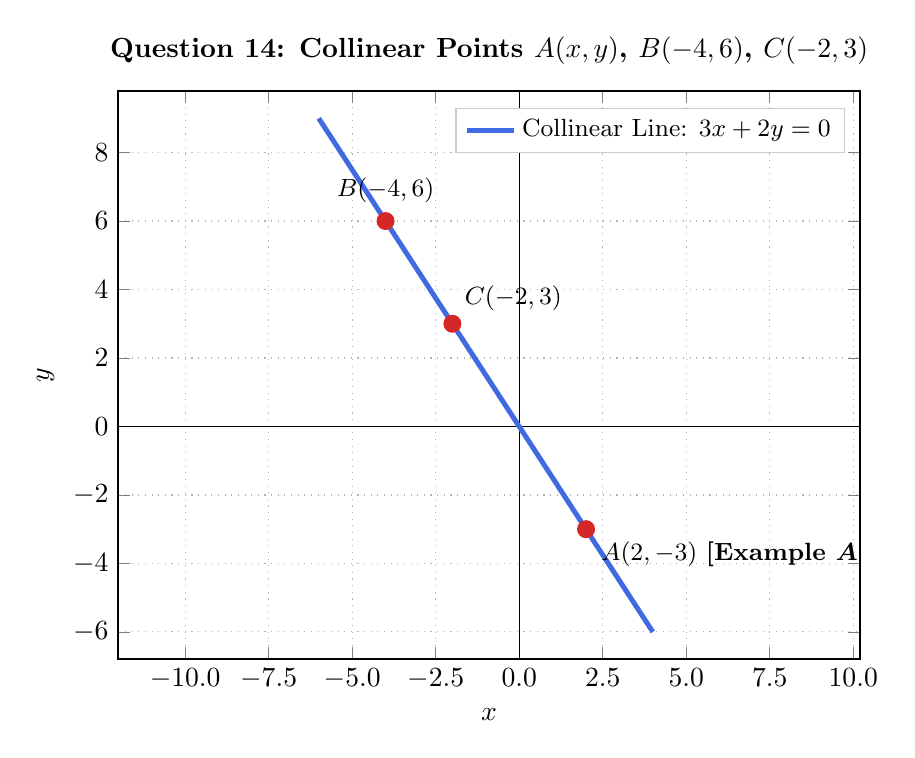
\begin{tikzpicture}
		\begin{axis}[
			width=11cm, height=8.8cm,
			title={\textbf{Question 14: Collinear Points $A(x, y)$, $B(-4, 6)$, $C(-2, 3)$}},
			xlabel={$x$}, ylabel={$y$},
			xmin=-12.0, xmax=10.2,
			ymin=-6.8, ymax=9.8,
			xtick={-10.0,-7.5,-5.0,-2.5,0.0,2.5,5.0,7.5,10.0},
			xticklabel style={
				/pgf/number format/fixed,
				/pgf/number format/precision=1,
				/pgf/number format/zerofill
			},
			ytick={-6,-4,-2,0,2,4,6,8},
			grid=both,
			grid style={dotted, gray!60},
			axis line style={black, thick},
			legend cell align={left},
			legend style={at={(0.98,0.97)}, anchor=north east, font=\small, draw=gray!40}
			]
			% Origin axis lines
			\draw[black, thin] (axis cs:0,-6.8) -- (axis cs:0,9.8);
			\draw[black, thin] (axis cs:-12,0) -- (axis cs:10.2,0);
			
			% Collinear line: 3x + 2y = 0  =>  y = -1.5x (from x = -6 to x = 4)
			\addplot[plotblue, line width=1.8pt, domain=-6:4, samples=2] {-1.5*x};
			\addlegendentry{Collinear Line: $3x + 2y = 0$}
			
			% Point B(-4, 6)
			\node[circle, fill=dotred, inner sep=2.3pt] at (axis cs:-4,6) {};
			\node[above=3pt, anchor=south, font=\small] at (axis cs:-4,6) {$B(-4, 6)$};
			
			% Point C(-2, 3)
			\node[circle, fill=dotred, inner sep=2.3pt] at (axis cs:-2,3) {};
			\node[above right=1pt, anchor=south west, font=\small] at (axis cs:-2,3) {$C(-2, 3)$};
			
			% Point A(2, -3)
			\node[circle, fill=dotred, inner sep=2.3pt] at (axis cs:2,-3) {};
			\node[anchor=north west, font=\small, xshift=2pt, yshift=-1pt] at (axis cs:2,-3) {$A(2, -3)$ \textbf{[Example \boldmath$A(x, y)$]}};
		\end{axis}
	\end{tikzpicture}
\end{document}